\section{Resultados}
A continuación se muestran algunas imágenes obtenidas del simulador del péndulo simple.



\begin{figure}[hb]
 \centering 
 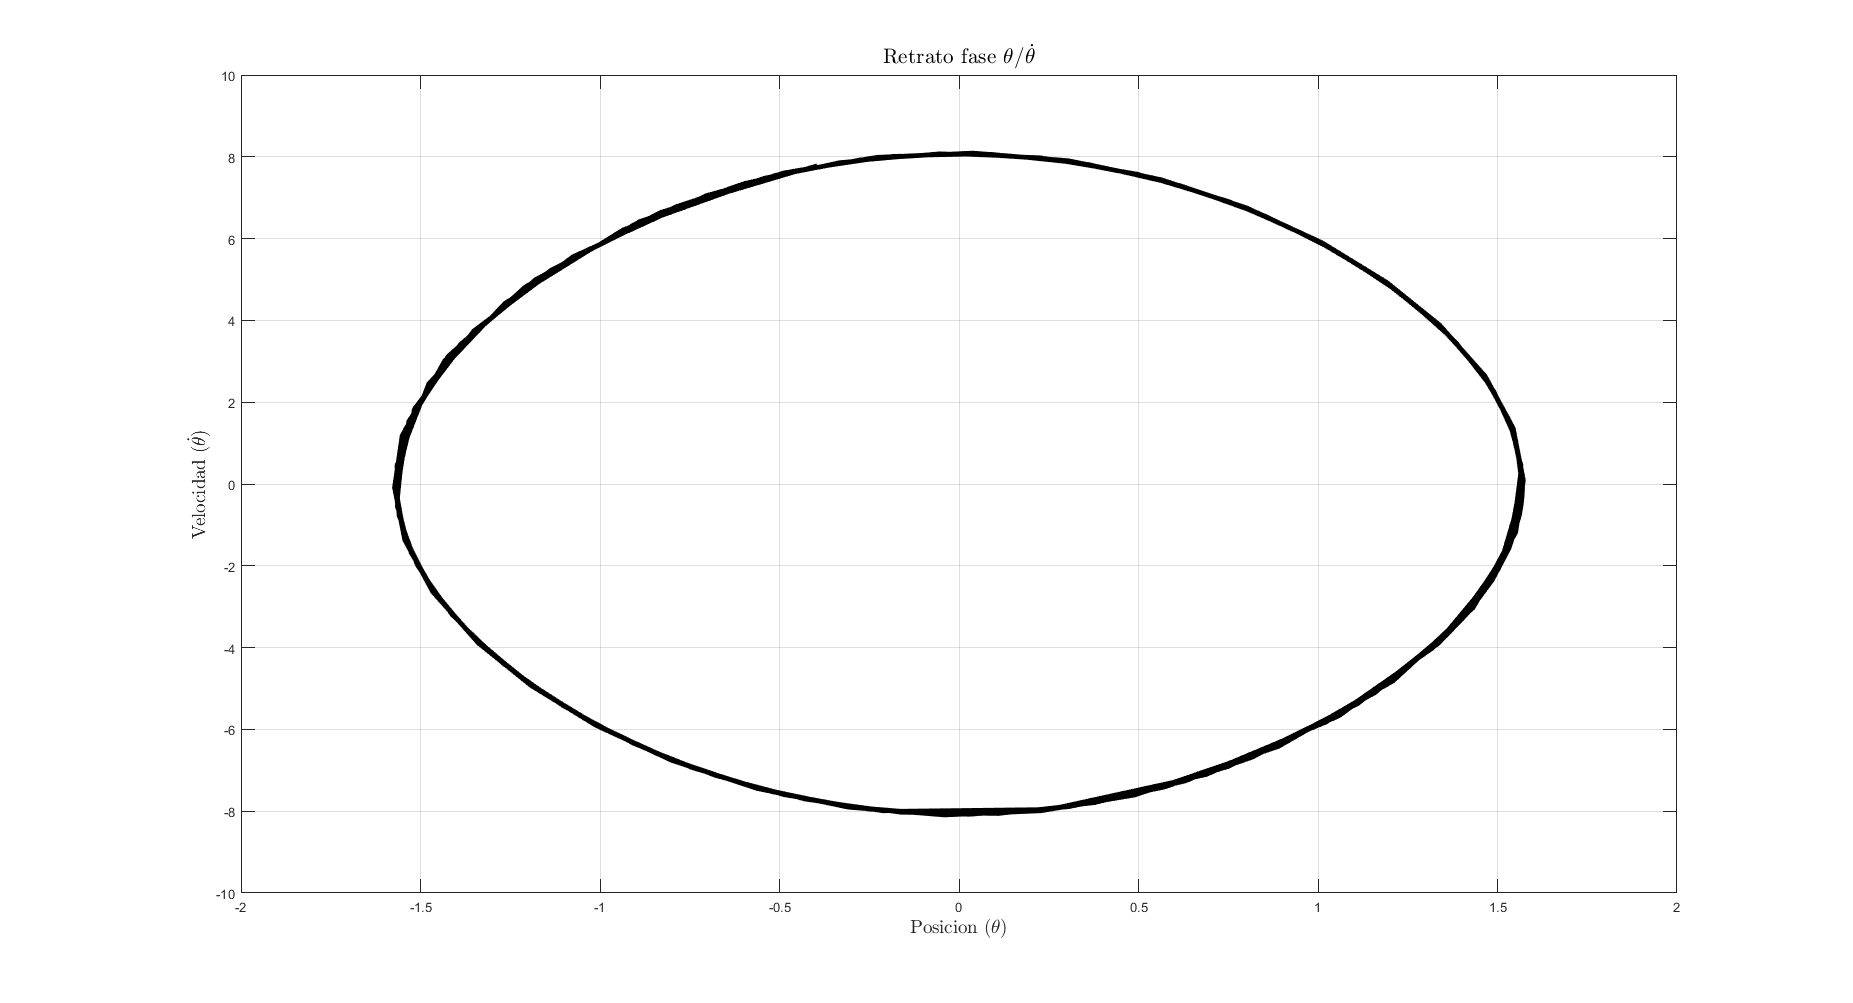
\includegraphics[scale=0.35]{./img/faseNF.png}
 % fasependulox2.png: 1853x1003 px, 96dpi, 49.02x26.53 cm, bb=0 0 1390 752
\caption{Diagrama de fase de $\theta(t)$ y $\dot{\theta}(t)$.}
 \label{fig: phase plot - NF}
\end{figure}

Podemos observar la figura de un circulo. Esto ocurre, porque el sistema no tiene fricción, no existe una fuerza que detenga el movimiento, ni disminuya la velocidad del péndulo, por lo cual tenemos un movimiento armónico simple.\\

En la figura \ref{fig: time plot - NF} se representa la posición y velocidad del péndulo en el tiempo.

\begin{figure}[hb]
 \centering 
 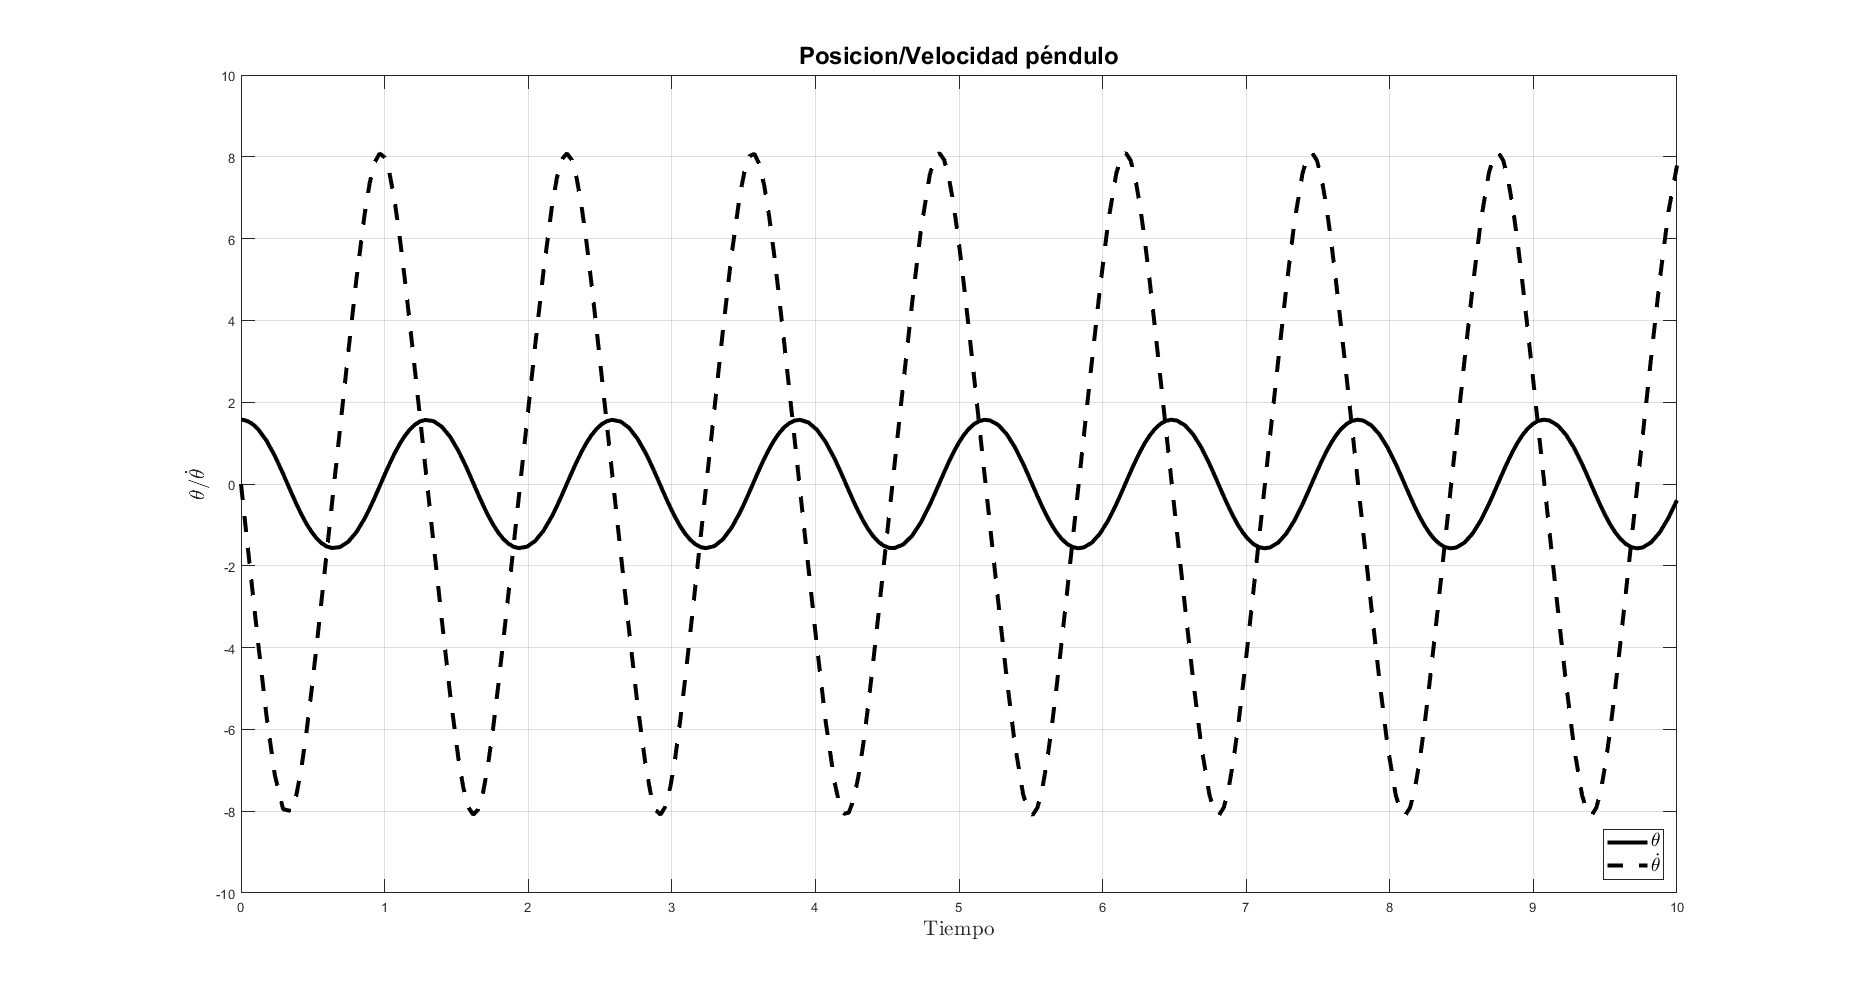
\includegraphics[scale=0.35]{./img/PosVelNF.png}
 % fasependulox2.png: 1853x1003 px, 96dpi, 49.02x26.53 cm, bb=0 0 1390 752
 \caption{Comportamiento de $\theta(t)$ y $\dot{\theta}(t)$ en el tiempo.}
 \label{fig: time plot - NF}
\end{figure}

Al ser un movimiento armónico, la posición y velocidad se comportan de manera periódica, oscilando entre valores de $\frac{\pi}{2}$ y $-\frac{\pi}{2}$ para la posición y entre $8$ y $-8$ radianes para la velocidad. Ya que el sistema no tiene una fuerza que se oponga el movimiento, no tiene una manera de disipar la energía del sistema, el péndulo continuara moviéndose hasta que una fuerza externa lo detenga.\\


En la figura \ref{fig: phase plot - F} se representa el diagrama fase del sistema para posición y velocidad del péndulo con respecto al angulo $\theta$. A diferencia de las imágenes anteriores, que no estaba presente la fricción, en las siguientes la fricción esta presente en nuestro sistema. Podemos observar que la velocidad y la posición comienzan a converger en cero. Lo que significa que el péndulo esta comenzado a detenerse. La velocidad tiende a $0$ y el péndulo tiende a estar en una posición de $0°$.

\begin{figure}[hb]
 \centering 
 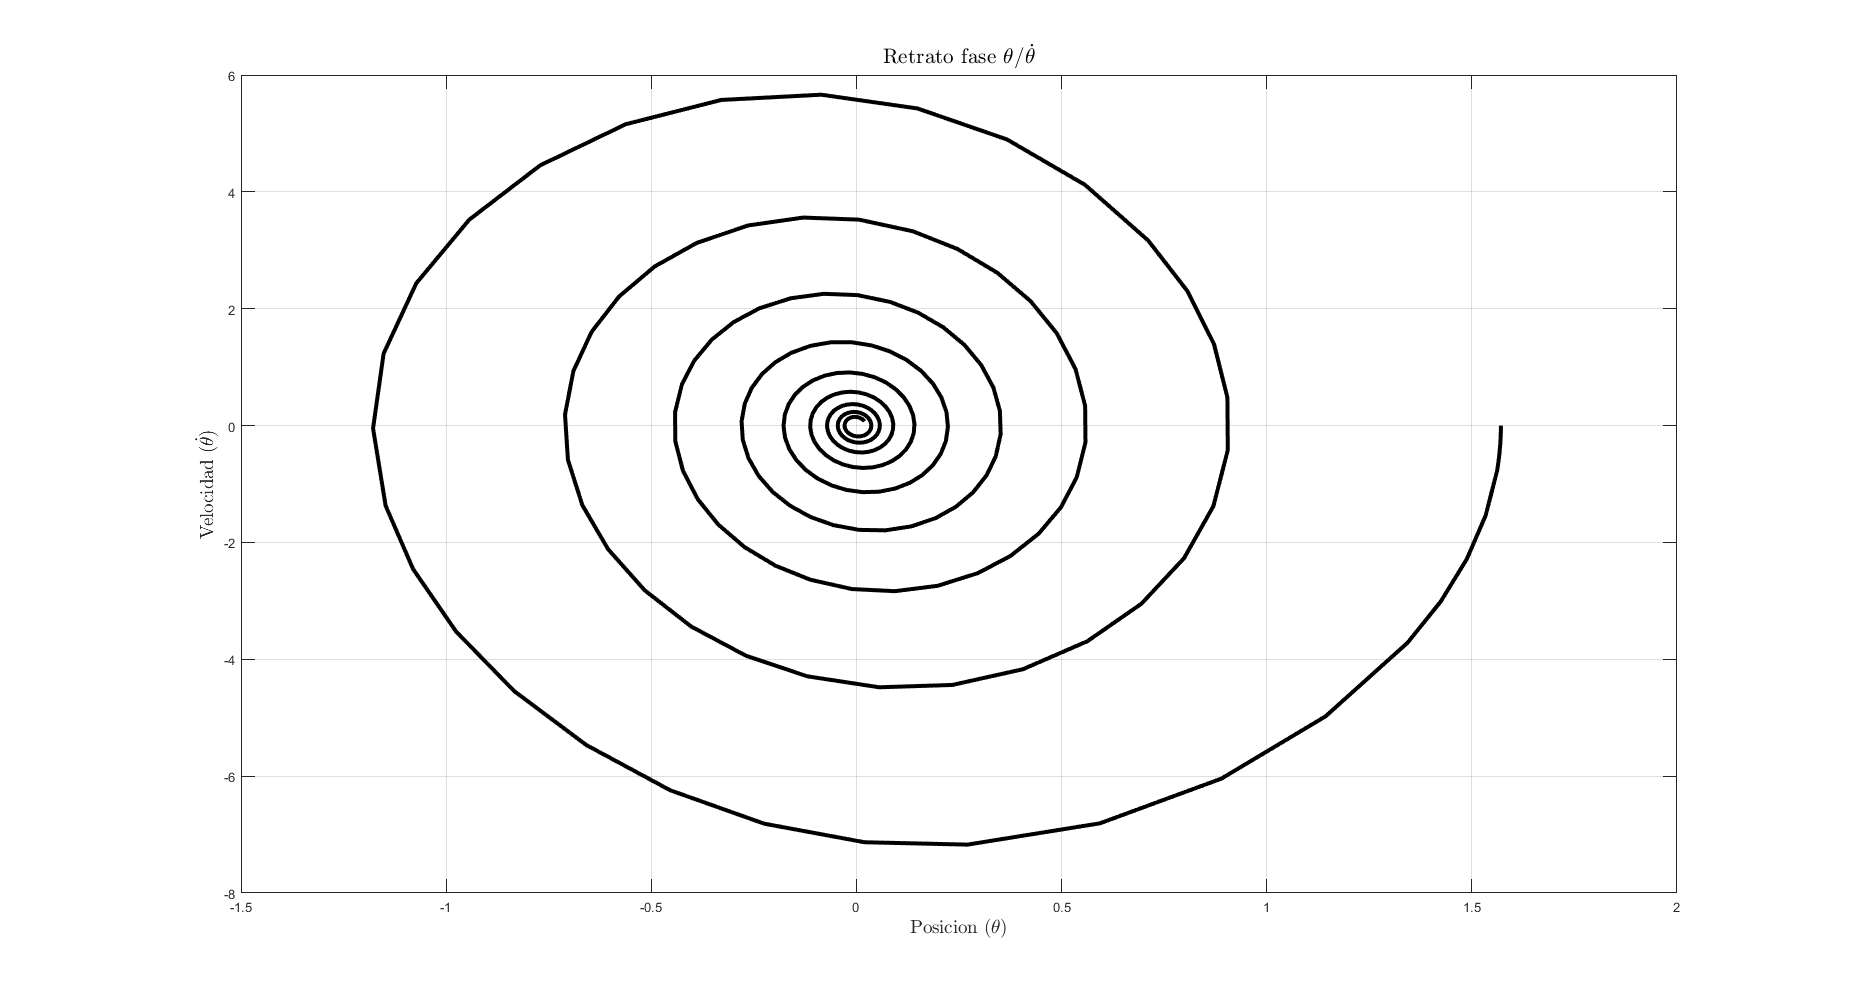
\includegraphics[scale=0.35]{./img/faseF.png}
 % fasependulox2.png: 1853x1003 px, 96dpi, 49.02x26.53 cm, bb=0 0 1390 752
\caption{Diagrama de fase de $\theta(t)$ y $\dot{\theta}(t)$.}
 \label{fig: phase plot - F}
\end{figure}




\begin{figure}[hb]
 \centering 
 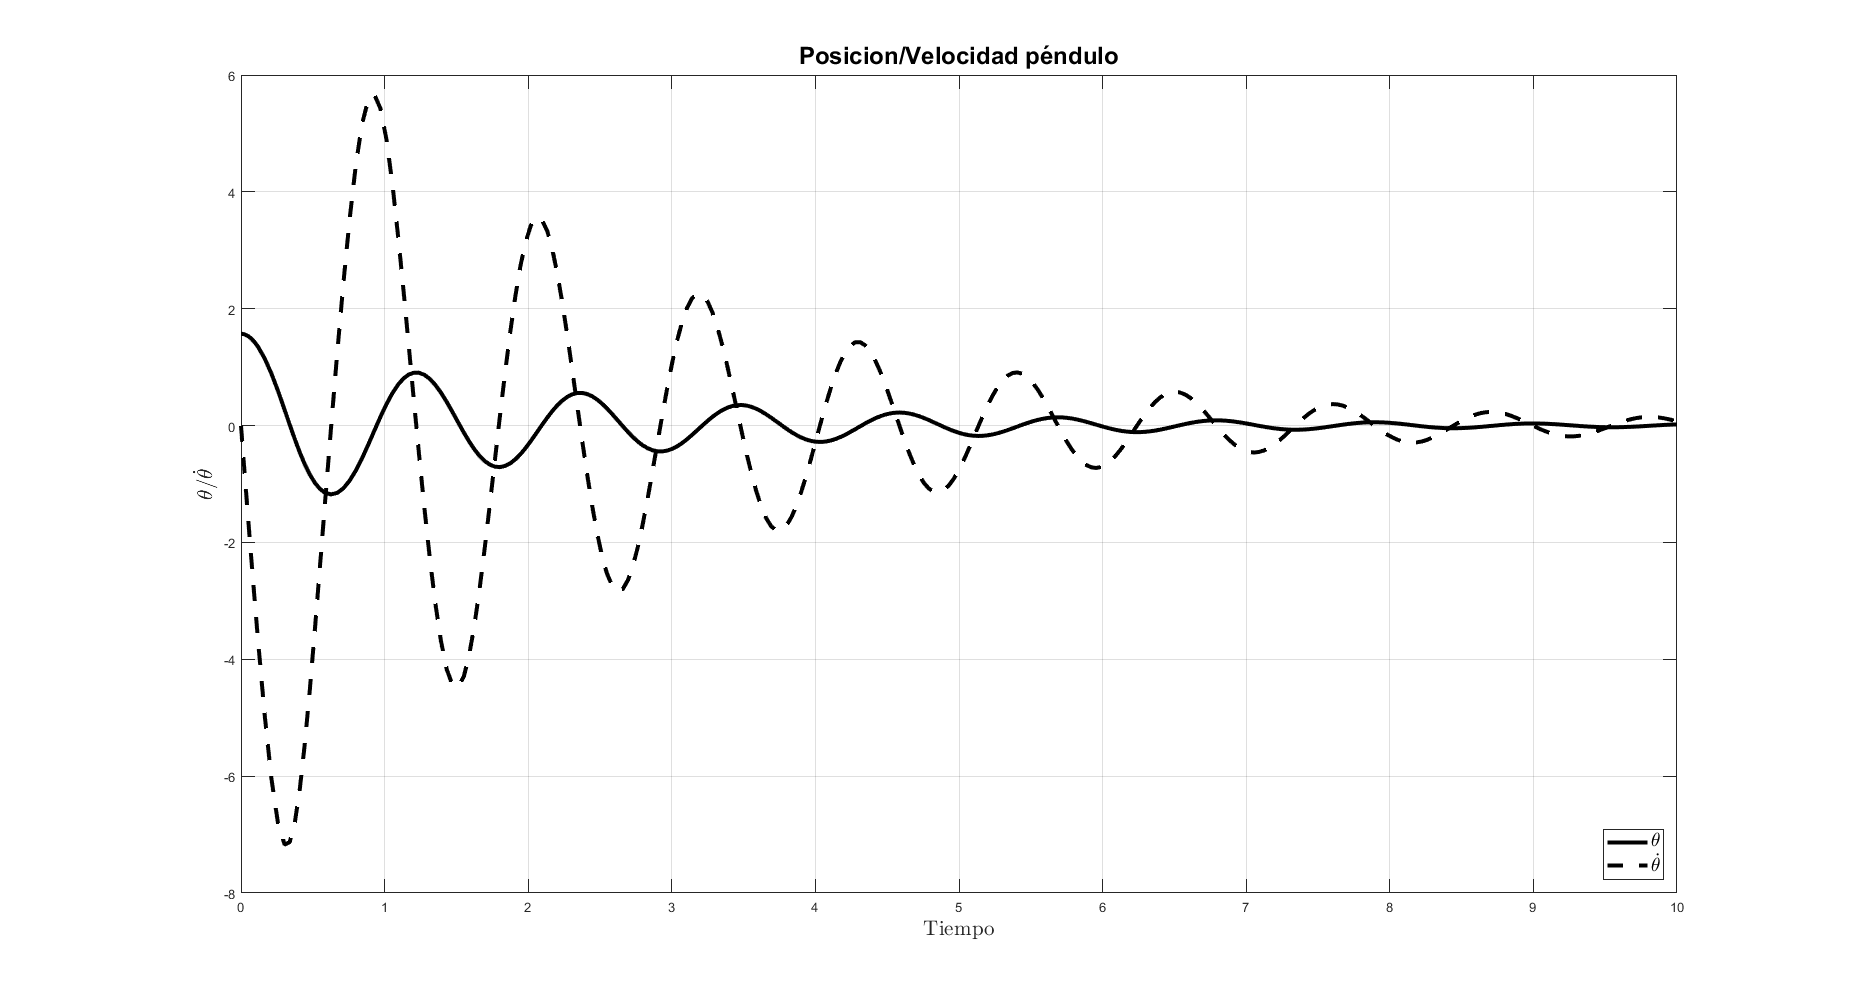
\includegraphics[scale=0.35]{./img/PosVelF.png}
 % fasependulox2.png: 1853x1003 px, 96dpi, 49.02x26.53 cm, bb=0 0 1390 752
 \caption{Comportamiento de $\theta(t)$ y $\dot{\theta}(t)$ en el tiempo.}
 \label{fig: time plot - F}
\end{figure}



\begin{figure}[h]
 \centering
 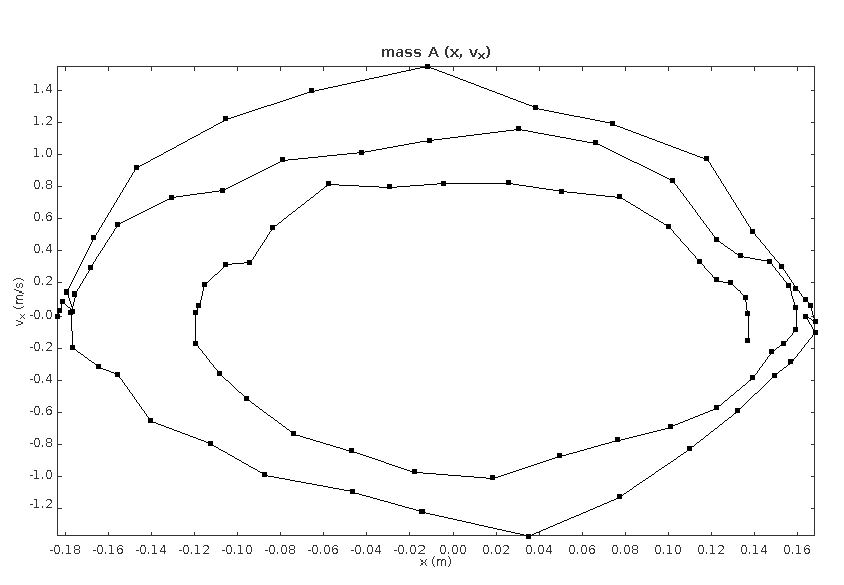
\includegraphics[scale=0.45]{./img/tracker_poc_phasediagram_x_vx.png}
 % tracker_poc_phasediagram_x_vx.png: 844x585 px, 72dpi, 29.78x20.64 cm, bb=0 0 844 585
 \caption{Diagrama de fase del modelo físico para $x$ y $\dot{x}$}
 \label{fig: tracker phase diagram x vx}
\end{figure}

\begin{figure}[h]
 \centering
 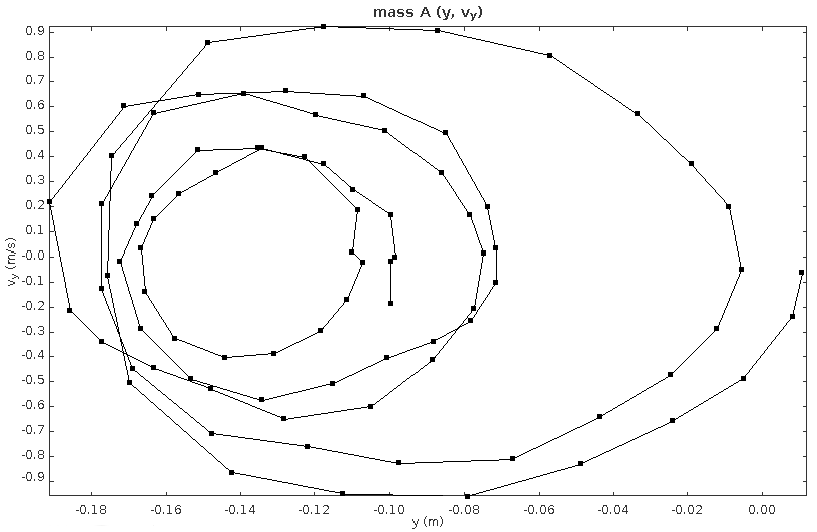
\includegraphics[scale=0.45]{./img/tracker_poc_phasediagram_y_vy.png}
 % tracker_poc_phasediagram_x_vx.png: 844x585 px, 72dpi, 29.78x20.64 cm, bb=0 0 844 585
 \caption{Diagrama de fase del modelo físico para $y$ y $\dot{y}$}
 \label{fig: tracker phase diagram y vy}
\end{figure}


\begin{figure}[h]
 \centering
 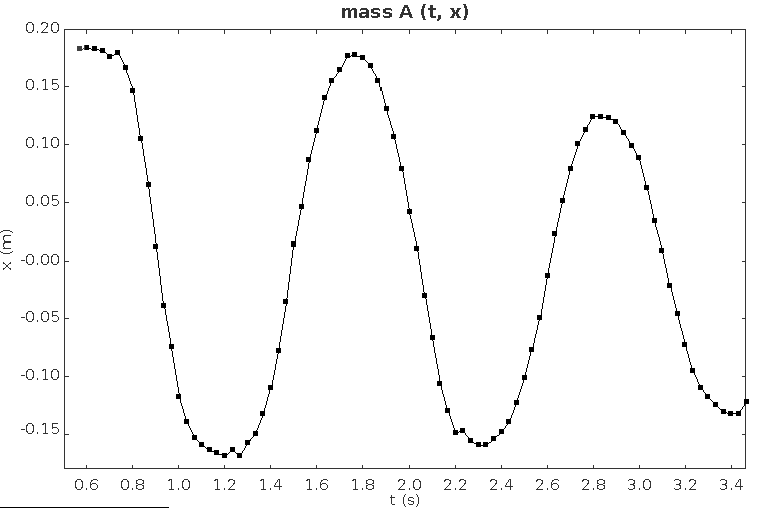
\includegraphics[scale=0.3]{./img/tracker_poc_timeplot_x.png}
 % tracker_poc_phasediagram_x_vx.png: 844x585 px, 72dpi, 29.78x20.64 cm, bb=0 0 844 585
 \caption{Diagrama de tiempo del modelo físico para $x$.}
 \label{fig: tracker time diagram x}
\end{figure}
